\documentclass[11pt,a4paper]{article}
\usepackage[T1]{fontenc}
\usepackage{lmodern}
\usepackage[margin=25mm]{geometry}
\usepackage{amsmath,amssymb,amsthm,mathtools}
\usepackage{booktabs,array}
\usepackage{xcolor}
\usepackage{tikz}
\usetikzlibrary{positioning,arrows.meta,decorations.pathreplacing,calc,fit,backgrounds}
\usepackage{pgfplots}
\pgfplotsset{compat=1.18}
\usepackage[ruled,vlined,linesnumbered]{algorithm2e}
\usepackage{enumitem}
\usepackage{microtype}
\usepackage[hidelinks]{hyperref}
\usepackage{xurl}
\usepackage[capitalise,noabbrev]{cleveref}

\definecolor{accent}{HTML}{C0392B}
\definecolor{ink}{HTML}{1F3A5F}
\definecolor{soft}{HTML}{DCE6F2}
\definecolor{core}{HTML}{2E86AB}
\definecolor{leaf}{HTML}{E9A23B}

\newtheorem{theorem}{Theorem}[section]
\newtheorem{lemma}[theorem]{Lemma}
\newtheorem{proposition}[theorem]{Proposition}
\newtheorem{corollary}[theorem]{Corollary}
\theoremstyle{definition}
\newtheorem{definition}[theorem]{Definition}
\newtheorem{remark}[theorem]{Remark}
\newtheorem{observation}[theorem]{Observation}

\newcommand{\Q}{\mathcal{Q}}
\newcommand{\N}{N}
\newcommand{\cN}{N[}
\newcommand{\PeelRatio}{5.1}
\newcommand{\QfiveSnake}{0, 1, 3, 7, 15, 14, 12, 28, 29, 25, 27, 26, 18, 22}
\newcommand{\QfiveTrans}{0123014021032}
\newcommand{\WinSnake}{0}
\newcommand{\WinI}{145}
\newcommand{\WinJ}{186}
\newcommand{\WinA}{422}
\newcommand{\WinB}{53}
\newcommand{\WinDiff}{2}
\newcommand{\KeepCFourDone}{35}
\newcommand{\regrowcoords}{(64,1.351e+05) (72,1.245e+06) (80,2.063e+07) (88,1.703e+08)}
\newcommand{\ComboJobs}{2{,}105}
\newcommand{\ComboWindows}{6{,}315}
\newcommand{\ComboFillings}{527{,}838{,}115}
\newcommand{\ComboWinUnknown}{1{,}520}
\newcommand{\ComboSeconds}{1525}

\makeatletter\newcommand{\rows}[1]{\@@input #1 }\makeatother

\title{Exhaustive Bitset Search for Long Snakes in the Nine-Cube:\\
Pruning Bounds, Rigidity, and Combined Moves}
\author{Yichen Zhan}
\date{15 October 2026}

\begin{document}
\maketitle

\begin{abstract}
The largest number of edges $a(9)$ of an induced path (a \emph{snake}) in the nine-dimensional hypercube is known only to satisfy $191\le a(9)\le 245$. A verified 192-edge snake would improve the lower bound. This report develops an exhaustive search engine for this question and applies it to the 131 published 191-edge snakes. The engine combines 512-bit bitset path growth with two provably valid pruning bounds: a parity-alternation bound and a new \emph{leaf-peeling} bound. The peeling bound shows that a path entering a tree-like part of the free region must end there, which reduces search nodes by a factor of about \PeelRatio. Four contributions follow.
(i)~A parity obstruction: internal rewiring alone can never produce a 192-edge snake, so any improvement must change an end.
(ii)~Exhaustive end regrowth: with the first 112 vertices of either end of any bank snake fixed, no 192-edge snake exists. This covers all $262$ instances with up to 80 freed vertices; earlier searches reached 40.
(iii)~Rigidity: 84\% of sixty-vertex internal windows admit exactly one filling, and 86\% of the alternatives are single square flips.
(iv)~A combined \emph{truncate--shorten--regrow} move, which tested $5.3\times10^{8}$ modified snakes and found no improvement.
A Lean development makes part of this machine-checked. The parity obstruction is proved for the project's own snake definition. A kernel-friendly exhaustive search, with verified parity and leaf-peeling bounds, is proved sound. With it, the Lean kernel certifies that no 192-edge snake shares a 152-vertex end segment with any published 191-edge snake. In dimension eight, the known 98-edge snake admits no other optimal completion after 59 of its 99 vertices are freed. This suggests that optimal eight-dimensional snakes are rare, and that the single-crossing targets $196$ and $197$ could be decided by classification. All exclusions are exhaustive within stated restricted families. None is a certificate for the global optimum, and the bounds $191\le a(9)\le245$ are unchanged.
\end{abstract}

\tableofcontents

%======================================================================
\section{Context and goal}

Let $\Q_n$ be the hypercube graph on $\{0,1\}^n$; vertices are written as integers $0,\dots,2^n-1$. A \emph{snake} is a path $P=(p_0,\dots,p_m)$ in $\Q_n$ that is an induced subgraph: $p_i$ and $p_j$ are adjacent exactly when $|i-j|=1$. Its length is $m$, the number of edges. The maximum length $a(n)$ is known exactly for $n\le 8$, with $a(8)=98$~\cite{ostergard,oeis}. For $n=9$, published constructions reach $191$~\cite{orland,data}. A companion research checkpoint by Iori Hironaka and Tommy Ma proves $a(9)\le 245$ in Lean and conjectures, with low confidence, that $a(9)=196$.

This report addresses the construction branch of that project:
\begin{quote}\itshape
Search for structurally different longer constructions. A verified 192-edge snake would already improve the lower bound. Promising routes include different eight-dimensional seeds, multiple crossings between layers, and asymmetric induced cycles. Compatible layer paths of lengths 98 and 97 would yield 196; lengths 98 and 98 would yield 197.
\end{quote}
Before this work, the main tools were Python depth-first regrowth, which could free at most about 40 vertices, and CP-SAT models; the joint layer models timed out. The contributions here are a fast exact engine (\cref{sec:engine,sec:bounds}), a structural obstruction (\cref{sec:parity}), and four families of experiments (\cref{sec:regrow,sec:rigid,sec:combo,sec:q8}), with validation in \cref{sec:valid}.

\begin{remark}[Status of claims]
\emph{Proved} results (Lemmas~\ref{lem:ban}, \ref{lem:parity} and~\ref{lem:peel}, and Proposition~\ref{prop:parity}) have complete proofs here. Proposition~\ref{prop:parity} and its corollary are also \emph{Lean-checked}, as are the end-regrowth exclusions with 160 and 152 fixed vertices for every bank snake (\cref{sec:lean}). The other \emph{computed} results come from exhaustive search: the program explored every branch not removed by a proved bound. Such results are reproducible but are not formally certified. Every reported path is re-verified independently by an all-pairs check.
\end{remark}

%======================================================================
\section{The search engine}\label{sec:engine}

\subsection{Bitset state}
Every subset of $V(\Q_9)$ is stored as eight 64-bit words. The program precomputes the open and closed neighbourhoods $\N(v)$ and $\N[v]=\N(v)\cup\{v\}$ for every vertex, together with the two parity classes $E$ (even weight) and $O$ (odd weight). A growing path is kept with its \emph{ban set}.

\begin{lemma}[Ban-set invariant]\label{lem:ban}
Let $P=(p_0,\dots,p_m)$ be a snake with head $h=p_m$, and let
\[
B(P)=\{h\}\cup\bigcup_{i<m}\N[p_i].
\]
For $x\in\N(h)$, the path $(p_0,\dots,p_m,x)$ is a snake if and only if $x\notin B(P)$. Moreover $B(P,x)=B(P)\cup\N[h]$.
\end{lemma}

\begin{proof}
The extended path is induced exactly when $x$ is new and is adjacent to no $p_i$ with $i<m$; that is, $x\notin\{p_m\}\cup\bigcup_{i<m}\N[p_i]$. The update formula is the definition with $m$ replaced by $m+1$.
\end{proof}

Each extension step therefore costs one 512-bit \textsc{or}. The candidate moves are the at most nine neighbours of $h$ outside $B$.

\subsection{Exhaustive regrowth}
\Cref{alg:regrow} fixes a prefix (the first $K$ vertices of a known snake) and decides whether some extension reaches a target number $T$ of vertices. The upper bound $\mathrm{UB}$ of \cref{sec:bounds} is evaluated at every node. A branch is cut only when even the bound cannot reach $T$, so the answer is exact for the stated family: either a witness is printed, or the subtree is exhausted.

\begin{algorithm}[ht]
\caption{\textsc{Regrow}$(P,T)$: does some snake extending $P$ have $\ge T$ vertices?}\label{alg:regrow}
\KwIn{snake prefix $P$ with head $h$; ban set $B=B(P)$; target $T$}
\If{$|P|\ge T$}{\Return \textsc{found}$(P)$}
$u\leftarrow \mathrm{UB}(h,B)$\tcp*{Lemmas~\ref{lem:parity} and~\ref{lem:peel}}
\If{$|P|+u<T$}{\Return \textsc{none}}
\ForEach{$x\in\N(h)\setminus B$}{
  \If{\textsc{Regrow}$\bigl(P\cdot x,\;B\cup\N[h]\bigr)$ found $Q$}{\Return \textsc{found}$(Q)$}
}
\Return \textsc{none}
\end{algorithm}

The same kernel supports three further modes:
\begin{itemize}[leftmargin=*]
\item \emph{window}: enumerate every induced replacement of an internal stretch (\cref{sec:rigid});
\item \emph{combo}: shorten a window, then regrow the end (\cref{sec:combo});
\item \emph{layer-restricted regrowth}: model single-crossing joins (\cref{sec:q8}).
\end{itemize}
An optional enumeration switch prints every solution instead of stopping at the first.

%======================================================================
\section{Two pruning bounds}\label{sec:bounds}

Fix a prefix with head $h$ and ban set $B$, and let $F=V\setminus B$ be the free vertices. Let $R\subseteq F$ be the set of free vertices reachable from $\N(h)\cap F$ inside $\Q_n[F]$. By Lemma~\ref{lem:ban}, every vertex $x_1,\dots,x_r$ of any extension lies in $F$. The extension is a path from $h$, so it lies in $R$. One breadth-first search computes $R$.

\subsection{Parity alternation}

\begin{lemma}[Parity bound]\label{lem:parity}
Let $R_{\neq}$ be the vertices of $R$ whose parity differs from $h$, and $R_{=}$ the rest. Every extension has
\[
r\;\le\;\min\bigl(|R_{\neq}|,\,|R_{=}|+1\bigr)\;+\;\min\bigl(|R_{=}|,\,|R_{\neq}|\bigr).
\]
\end{lemma}

\begin{proof}
$\Q_n$ is bipartite, so $x_i$ has the parity of $h$ exactly when $i$ is even. The odd-indexed vertices number $\lceil r/2\rceil$ and lie in $R_{\neq}$. The even-indexed ones number $\lfloor r/2\rfloor$ and lie in $R_{=}$. Since $\lfloor r/2\rfloor\le\lceil r/2\rceil\le\lfloor r/2\rfloor+1$, we get $\lceil r/2\rceil\le\min(|R_{\neq}|,|R_=|+1)$ and $\lfloor r/2\rfloor\le\min(|R_=|,|R_{\neq}|)$. Add the two inequalities.
\end{proof}

\subsection{Leaf peeling (new)}

The parity bound ignores shape. Near the end of a long snake the free region is often tree-like, and a path cannot enter a dangling tree and come back out. The second bound turns this into an exact inequality.

\begin{definition}[Peeling]\label{def:peel}
Let $G=\Q_n[R\cup\{h\}]$. Put every $x\in R$ with $\deg_G(x)\le1$ into a FIFO queue with label $\lambda(x)=1$. Repeatedly pop a vertex $u$ and decrement the current degree of each not-yet-queued neighbour $x\in R$ (never $h$). When that degree drops to at most $1$, enqueue $x$ with $\lambda(x)=\lambda(u)+1$. Let $D$ be the set of vertices ever queued, $C=R\setminus D$ the \emph{core}, and $\lambda_{\max}=\max_D\lambda$ (zero if $D=\emptyset$).
\end{definition}

The procedure has two properties, both immediate from the construction. Labels are non-decreasing in queue order, because each label is one more than the label of the vertex being popped.
\begin{enumerate}[label=(P\arabic*),leftmargin=*]
\item\label{P1} Each $x\in D$ has at most one neighbour in $G$ that was not popped before $x$ was enqueued. Vertices of $C\cup\{h\}$ are never popped.
\item\label{P2} Every neighbour $w$ of $x$ that was popped before $x$ was enqueued satisfies $\lambda(w)\le\lambda(x)-1$. Indeed, $x$ was enqueued while some $u$ was being popped, $\lambda(x)=\lambda(u)+1$, and every vertex popped up to that moment has label at most $\lambda(u)$.
\end{enumerate}

\begin{lemma}[Leaf-peeling bound]\label{lem:peel}
Every extension $(x_1,\dots,x_r)$ satisfies $r\le |C|+\lambda_{\max}$.
\end{lemma}

\begin{proof}
If no $x_i$ lies in $D$, then $r\le|C|$. Otherwise let $s$ be the least index with $x_s\in D$, and write $x_0=h$. The claim is that for every $i\ge s$, $x_i\in D$ and $x_{i+1}$ (if it exists) was popped before $x_i$ was enqueued.

Start with $i=s$. The predecessor $x_{s-1}$ lies in $C\cup\{h\}$ and is never popped. By \ref{P1} it is the only neighbour of $x_s$ not popped before $x_s$ was enqueued, so $x_{s+1}\ne x_{s-1}$ was popped earlier and hence lies in $D$.

For the inductive step, suppose $x_i$ was popped before $x_{i-1}$ was enqueued. Then $x_{i-1}$ had not been popped when $x_i$ was enqueued, so by \ref{P1} it is the unique such neighbour of $x_i$. Hence $x_{i+1}$ was popped before $x_i$ was enqueued.

By \ref{P2}, $\lambda(x_{s})>\lambda(x_{s+1})>\dots>\lambda(x_r)\ge1$, so at most $\lambda(x_s)\le\lambda_{\max}$ vertices of the path lie in $D$. The vertices $x_1,\dots,x_{s-1}$ lie in $C$. Hence $r\le|C|+\lambda_{\max}$.
\end{proof}

The engine uses $\mathrm{UB}=\min(\text{bound of Lemma~\ref{lem:parity}},\ \text{bound of Lemma~\ref{lem:peel}})$. Both bounds remain valid if $R$ is replaced by any superset, because their hypotheses only require the extension to lie in $R$. The implementation therefore does not trouble to exclude the other neighbours of $h$.

\begin{figure}[ht]
\centering
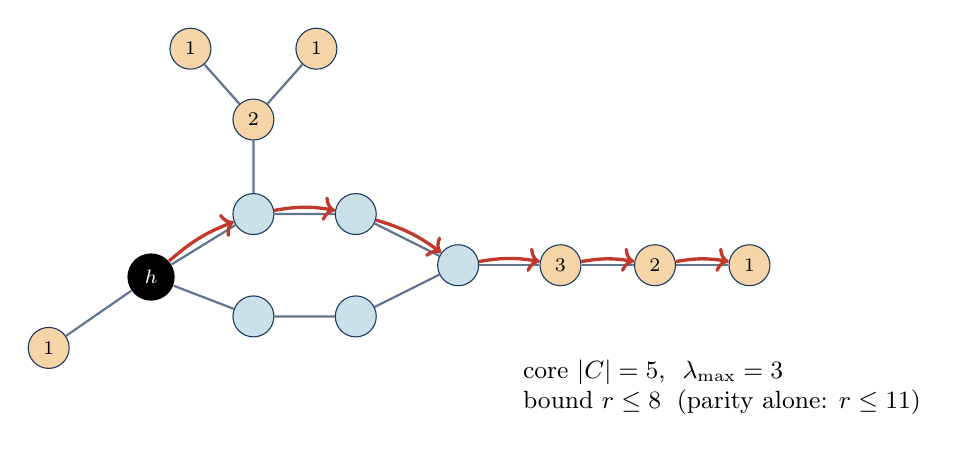
\begin{tikzpicture}[v/.style={circle,draw=ink,fill=core!25,minimum size=5.2mm,inner sep=0pt,font=\scriptsize},
  l/.style={circle,draw=ink,fill=leaf!45,minimum size=5.2mm,inner sep=0pt,font=\scriptsize},
  e/.style={draw=ink!70,thick}]
\node[circle,fill=black,text=white,minimum size=6mm,font=\scriptsize] (h) at (0,0) {$h$};
\node[v] (c1) at (1.3,0.8) {}; \node[v] (c2) at (2.6,0.8) {}; \node[v] (c3) at (2.6,-0.5) {}; \node[v] (c4) at (1.3,-0.5) {};
\node[v] (c5) at (3.9,0.15) {};
\draw[e] (h)--(c1) (h)--(c4) (c1)--(c2) (c3)--(c4) (c2)--(c5) (c3)--(c5);
% hanging path of height 3 from c5
\node[l] (a1) at (5.2,0.15) {3}; \node[l] (a2) at (6.4,0.15) {2}; \node[l] (a3) at (7.6,0.15) {1};
\draw[e] (c5)--(a1)--(a2)--(a3);
% hanging star of height 2 from c1
\node[l] (b1) at (1.3,2.0) {2}; \node[l] (b2) at (0.5,2.9) {1}; \node[l] (b3) at (2.1,2.9) {1};
\draw[e] (c1)--(b1) (b1)--(b2) (b1)--(b3);
% tree hanging from h
\node[l] (d1) at (-1.3,-0.9) {1};
\draw[e] (h)--(d1);
\draw[->,very thick,accent] (h) to[bend left=10] (c1);
\draw[->,very thick,accent] (c1) to[bend left=10] (c2);
\draw[->,very thick,accent] (c2) to[bend left=10] (c5);
\draw[->,very thick,accent] (c5) to[bend left=10] (a1);
\draw[->,very thick,accent] (a1) to[bend left=10] (a2);
\draw[->,very thick,accent] (a2) to[bend left=10] (a3);
\node[font=\small,align=left,anchor=west] at (4.6,-1.4) {core $|C|=5$,\ \ $\lambda_{\max}=3$\\ bound $r\le 8$ \;(parity alone: $r\le 11$)};
\end{tikzpicture}
\caption{Leaf peeling on a toy bipartite free region (core: the 6-cycle through $h$). Core vertices are blue, peeled vertices orange with their labels $\lambda$. A path from $h$ (red) can visit core vertices, but once it enters a peeled tree it can only descend, collecting at most $\lambda$ further vertices.}
\label{fig:peel}
\end{figure}

\paragraph{Effect.} \Cref{tab:bounds} compares the two bound configurations on identical exhaustive problems; the outcomes agree. Leaf peeling removes $\PeelRatio\times$ more nodes in total. Each node costs more, so the wall-clock gain is smaller (about $2\times$), but it grows with depth.

\begin{table}[ht]
\centering\small
\begin{tabular}{rrrrrrrl}
\toprule
$K$ & bank & nodes (parity) & nodes (+ peel) & ratio & s (parity) & s (+ peel) & outcome\\
\midrule
\rows{boundtable.tex}
\bottomrule
\end{tabular}
\caption{Regrowth to 193 vertices from the first $K$ vertices of bank snakes 0--3, forward orientation only. Outcomes agree, as they must, because both configurations are exact.}
\label{tab:bounds}
\end{table}

%======================================================================
\section{A parity obstruction for internal rewiring}\label{sec:parity}

\begin{proposition}\label{prop:parity}
Let $S$ be a snake in $\Q_n$ containing vertices $a=s_i$ and $b=s_j$ with $i<j$. Suppose the stretch $s_{i+1},\dots,s_{j-1}$ is replaced by any path from $a$ to $b$ such that the result $S'$ is again a snake. Then $|S'|-|S|$ is even.
\end{proposition}

\begin{proof}
In a bipartite graph, every walk from $a$ to $b$ has length congruent to $d(a,b)$ modulo $2$. The old and new stretches are both $a$--$b$ paths, so their lengths differ by an even number. Nothing else changes.
\end{proof}

\begin{corollary}\label{cor:end}
A snake obtained from a 191-edge snake by any sequence of internal replacements has odd length. In particular it is never of length $192$. A 192-edge snake that shares an internal skeleton with a known 191-edge snake must change at least one end.
\end{corollary}

This explains why the experiments below always free an end. It also identifies a hidden weakness of pure internal local search: the smallest improvement such a search can reach is $193$, not $192$.

\begin{figure}[ht]
\centering
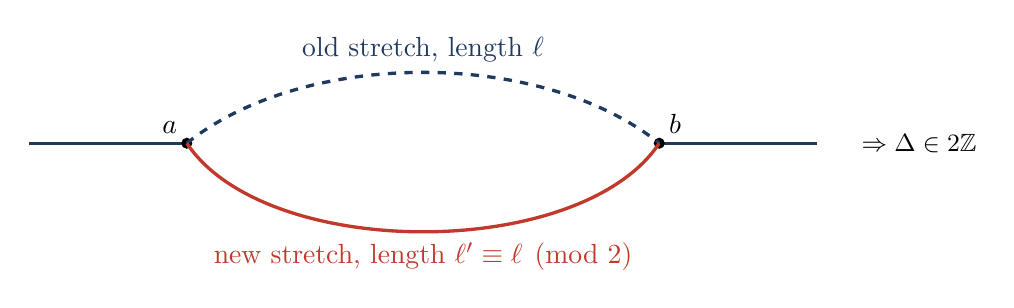
\begin{tikzpicture}[x=1cm,y=1cm]
\draw[very thick,ink] (0,0)--(2,0);
\draw[very thick,ink] (8,0)--(10,0);
\fill (2,0) circle (2pt) node[above left] {$a$};
\fill (8,0) circle (2pt) node[above right] {$b$};
\draw[very thick,ink,dashed] (2,0) .. controls (3.5,1.2) and (6.5,1.2) .. (8,0) node[pos=.5,above] {old stretch, length $\ell$};
\draw[very thick,accent] (2,0) .. controls (3,-1.5) and (7,-1.5) .. (8,0) node[pos=.5,below] {new stretch, length $\ell'\equiv\ell\pmod 2$};
\node[font=\small] at (11.3,0) {$\Rightarrow \Delta\in2\mathbb{Z}$};
\end{tikzpicture}
\caption{Internal rewiring between fixed vertices preserves the parity of the length (Proposition~\ref{prop:parity}).}
\end{figure}

%======================================================================
\section{Deep exhaustive end regrowth}\label{sec:regrow}

\paragraph{Model.} For each of the 131 bank snakes and each orientation (262 instances), fix the first $K$ vertices and run \cref{alg:regrow} with target $T=193$ vertices, that is, 192 edges. All new vertices are unrestricted in $\Q_9$, so any number of layer crossings is allowed. The runs used 12 workers on an Apple M5 Pro.

\begin{table}[ht]
\centering\small
\begin{tabular}{rrcrcccr}
\toprule
$K$ & freed & infeasible & unknown & total nodes & median & max & wall time\\
\midrule
\rows{regrowtable.tex}
\bottomrule
\end{tabular}
\caption{Exhaustive end regrowth over the whole bank. ``Freed'' is $192-K$, the number of original vertices released. $^\dagger$Run in progress with a cap of $5\times10^8$ nodes per instance; the entries shown are the instances finished when this report was generated. ``Unknown'' instances reached the cap and are unresolved.}
\label{tab:regrow}
\end{table}

\begin{figure}[ht]
\centering
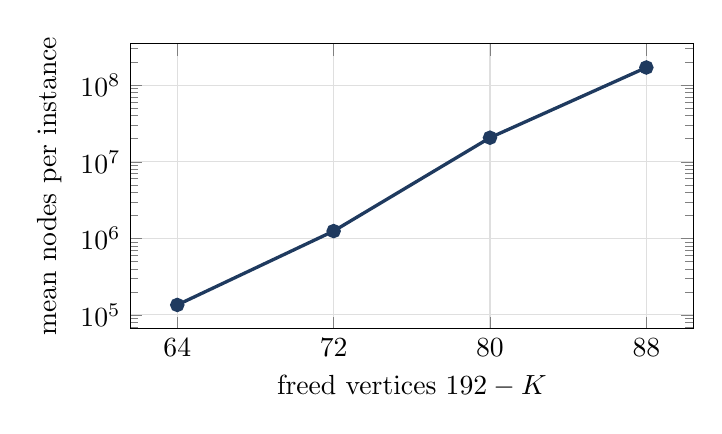
\begin{tikzpicture}
\begin{axis}[width=0.72\textwidth,height=5.2cm,ymode=log,xlabel={freed vertices $192-K$},
  ylabel={mean nodes per instance},xtick={64,72,80,88},grid=major,grid style={gray!25},
  every axis plot/.append style={very thick}]
\edef\regrowplotcmd{\noexpand\addplot[mark=*,color=ink] coordinates {\regrowcoords};}\regrowplotcmd
\end{axis}
\end{tikzpicture}
\caption{Search effort grows by roughly an order of magnitude for every eight freed vertices. The last point uses only the resolved instances of the running $K=104$ job.}
\label{fig:growth}
\end{figure}

\begin{observation}
No 192-edge snake shares a 112-vertex end segment with any of the 131 published 191-edge snakes. The earlier Python regrowth excluded only 152-vertex segments and left 53 instances at $K=144$ unresolved.
\end{observation}

%======================================================================
\section{Rigidity of internal windows}\label{sec:rigid}

\paragraph{Model.} Delete $W$ consecutive internal vertices $s_{i+1},\dots,s_{j-1}$ and enumerate every induced $a$--$b$ path ($a=s_i$, $b=s_j$) that rejoins the remaining snake. The ban set contains $\N[s_q]$ for every kept $q\notin\{i,j\}$, together with $a$ and $b$. The search closes as soon as the head becomes adjacent to $b$: an induced path cannot pass a neighbour of $b$ without stopping there. Equal-length fillings are \emph{plateau moves}. By Proposition~\ref{prop:parity} the only possible improvement is $+2$.

\begin{table}[ht]
\centering\small
\begin{tabular}{p{0.42\textwidth}cccc}
\toprule
& 1 filling & 2 fillings & 3 fillings & 4 fillings\\
\midrule
$W=60$, all 131 snakes, 4 windows each (524 windows, all exhausted) & 440 & 75 & 7 & 2\\
\bottomrule
\end{tabular}

\medskip
\begin{tabular}{lc}
\toprule
How an alternative filling differs from the original & count\\
\midrule
single square flip (2 transitions swapped, 1 vertex moved) & 82\\
double square flip (4 transitions, 2 vertices) & 2\\
genuinely different path (15--46 vertices differ) & 11\\
\bottomrule
\end{tabular}
\caption{Window rigidity. No window, at any size tested ($W=20$ to $80$), admitted a longer filling.}
\label{tab:rigid}
\end{table}

In smaller runs over windows of $W=30,40,50,60,80$, between 80\% and 86\% of windows were uniquely determined, and none admitted a $+2$ filling. When a window of 80 vertices (42\% of the snake) is deleted, the remaining 112 vertices usually force it back exactly.

\paragraph{Demonstration.} In bank snake \WinSnake, deleting the 40 vertices strictly between positions \WinI{} (vertex \WinA) and \WinJ{} (vertex \WinB) leaves exactly two fillings. Their transition sequences, with the \WinDiff{} differing digits highlighted, are
\begin{center}\small
\texttt{140132462132410231280123104312307603213\textcolor{accent}{\textbf{0}}\textcolor{accent}{\textbf{4}}}\\
\texttt{140132462132410231280123104312307603213\textcolor{accent}{\textbf{4}}\textcolor{accent}{\textbf{0}}}

\end{center}
This is a single square flip near $b$: the path turns $0,4$ instead of $4,0$, which moves one vertex across a 4-cycle.

\begin{figure}[ht]
\centering
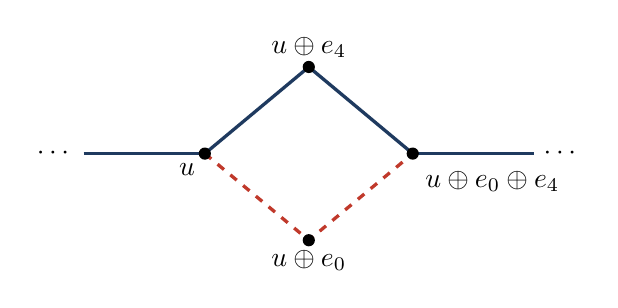
\begin{tikzpicture}[scale=1.1]
\coordinate (u) at (0,0); \coordinate (p) at (1.2,1.0); \coordinate (q) at (1.2,-1.0); \coordinate (w) at (2.4,0);
\draw[very thick,ink] (-1.4,0)--(u); \draw[very thick,ink] (w)--(3.8,0);
\draw[very thick,ink] (u)--(p)--(w);
\draw[very thick,accent,dashed] (u)--(q)--(w);
\foreach \x in {u,p,q,w} \fill (\x) circle (2pt);
\node[above] at (p) {$u\oplus e_4$}; \node[below] at (q) {$u\oplus e_0$};
\node[left] at (-1.4,0) {$\cdots$}; \node[right] at (3.8,0) {$\cdots$};
\node[below left] at (u) {$u$}; \node[below right=3pt and 1pt] at (w) {$u\oplus e_0\oplus e_4$};
\end{tikzpicture}
\caption{A square flip: the steps $(e_4,e_0)$ and $(e_0,e_4)$ give two routes around the same 4-cycle. Most plateau freedom in bank snakes is of this trivial kind.}
\end{figure}

\paragraph{Consequence.} Random walks on the plateau of 191-edge snakes through internal moves barely move: the bank consists of nearly isolated points. Diversity must come from the ends or from new constructions.

%======================================================================
\section{Combined truncate--shorten--regrow moves}\label{sec:combo}

Corollary~\ref{cor:end} and the rigidity results suggest a move that changes the interior and an end together. Shortening an internal stretch by two edges frees space. If that space lets the end grow by three or more, the total gains.

\begin{algorithm}[ht]
\caption{\textsc{Combo}$(S,\ \mathrm{CUT},W,\sigma,T)$}\label{alg:combo}
$S'\leftarrow(s_0,\dots,s_{\mathrm{CUT}-1})$\tcp*{drop the end}
choose a random internal window $(s_i,s_j)$ of $S'$ with $j-i=W+1$\;
\ForEach{induced $s_i$--$s_j$ filling $F$ of length $\ge (j-i)-2\sigma$}{
  $S''\leftarrow s_0\cdots s_i\,F\,s_j\cdots s_{\mathrm{CUT}-1}$\;
  \If{\textsc{Regrow}$(S'',T)$ finds $Q$}{\Return $Q$ (verify independently)}
}
\end{algorithm}

\begin{figure}[ht]
\centering
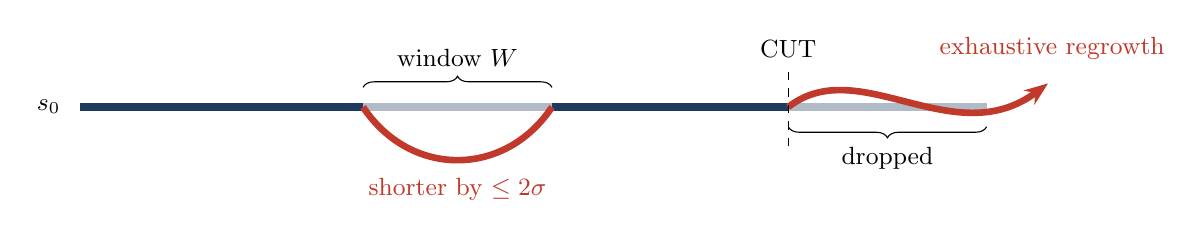
\begin{tikzpicture}[x=0.06cm,y=1cm]
\draw[line width=3pt,ink!35] (0,0)--(192,0);
\draw[line width=3pt,ink] (0,0)--(60,0); \draw[line width=3pt,ink] (100,0)--(150,0);
\draw[line width=2.4pt,accent] (60,0) .. controls (70,-0.9) and (90,-0.9) .. (100,0);
\draw[line width=2.4pt,accent,-{Stealth[length=3mm]}] (150,0) .. controls (165,0.7) and (185,-0.6) .. (205,0.3);
\draw[decorate,decoration={brace,amplitude=4pt}] (60,0.25)--(100,0.25) node[midway,above=4pt,font=\small] {window $W$};
\draw[decorate,decoration={brace,amplitude=4pt,mirror}] (150,-0.25)--(192,-0.25) node[midway,below=4pt,font=\small] {dropped};
\node[font=\small,accent] at (80,-1.05) {shorter by $\le2\sigma$};
\node[font=\small,accent,anchor=west] at (180,0.75) {exhaustive regrowth};
\node[font=\small,anchor=east] at (-2,0) {$s_0$};
\draw[dashed] (150,-0.5)--(150,0.5) node[above,font=\small] {CUT};
\end{tikzpicture}
\caption{A combined move. Blue: kept skeleton. Red: replaced parts.}
\end{figure}

\paragraph{Run.} The run used seed 1, \ComboSeconds\,s on 12 workers, $\mathrm{CUT}\in[140,180]$, $W\in[16,48]$, $\sigma\in\{1,2\}$ and both orientations of all 131 snakes. It covered \ComboJobs{} jobs and \ComboWindows{} windows, and \ComboFillings{} fillings were each followed by an exhaustive regrowth. No regrowth reached its node cap of $2\times10^5$. Some window enumerations, \ComboWinUnknown{} of them, reached their own cap of $2\times10^7$ nodes and were therefore covered only partly.

\begin{table}[ht]
\centering\small
\begin{tabular}{lrrrr}
\toprule
CUT range & windows & fillings tested & windows exhausted & 192-edge snakes\\
\midrule
\rows{combotable.tex}
\bottomrule
\end{tabular}
\caption{Combined moves by truncation depth. Deeper truncation leaves far more freedom in the window: nearly a hundred times more fillings at $\mathrm{CUT}\le150$ than at $\mathrm{CUT}>170$.}
\end{table}

This is a random sample of an enormous neighbourhood and implies no exclusion. Its main lesson is that even when the interior is loosened, the bounds of Lemmas~\ref{lem:parity} and~\ref{lem:peel} kill almost every regrowth immediately: regrowths averaged $1.005$ nodes, so more than 99.5\% were pruned at their root.

%======================================================================
\section{Eight-dimensional seeds and single crossings}\label{sec:q8}

\subsection{Encoding the joint layer problem as regrowth}
Write $\Q_9=\Q_8\times\Q_1$. Let $A$ be a snake in $\Q_8$ ending at $v$, and $B$ a snake in $\Q_8$ starting at $v$. Taylor~\cite{taylor} and the Lean module of the companion project show that
\[
A\times\{0\}\;\to\;(v,1)\;\to\;B\times\{1\}
\]
is a snake of length $|A|+|B|+1$ if and only if $A\cap B=\{v\}$.

\begin{lemma}\label{lem:layer}
Run \cref{alg:regrow} on the prefix $A\times\{0\}$ followed by $(v,1)$, with new vertices restricted to the layer $x_8=1$. It finds exactly the paths $B$ of the form above.
\end{lemma}

\begin{proof}
The ban set contains $\N[(a,0)]\ni(a,1)$ for every $a\in A\setminus\{v\}$. A vertex $(b,1)$ is therefore admissible exactly when $b\notin A\setminus\{v\}$ and the layer-1 path stays induced, which is the compatibility condition.
\end{proof}

\paragraph{Partner probe.} For the published 98-edge Carlson--Hougen seed~\cite{records}, the search for a 97-edge partner at endpoint 78 returned \emph{unknown} after $3\times10^9$ nodes (6206\,s). In this setting the free region has about 157 vertices and is not tree-like, so neither bound is strong. The exact maximum partner length for this seed therefore remains open.

\subsection{The 98-edge seed is isolated}
Using the enumeration switch, the search fixed the first $K$ vertices of the 98-edge seed and listed \emph{every} completion to 98 edges in $\Q_8$, in both orientations.

\begin{table}[ht]
\centering\small
\begin{tabular}{rrcr}
\toprule
$K$ fixed & vertices freed & completions (fwd, rev) & nodes (fwd, rev)\\
\midrule
70 & 29 & 1, 1 & 147, 50\\
60 & 39 & 1, 1 & 212, 2{,}180\\
50 & 49 & 1, 1 & 794, 5{,}793\\
40 & 59 & 1, 1 & $7.9\times10^{7}$, $6.5\times10^{5}$\\
\bottomrule
\end{tabular}
\caption{Every optimal completion of a prefix of the known 98-edge $\Q_8$ snake. The only completion is the seed itself.}
\end{table}

\begin{observation}
Freeing 59 of its 99 vertices does not produce a second optimal $\Q_8$ snake. Optimal eight-dimensional snakes thus appear to be sparse and mutually far apart. ``Different eight-dimensional seeds'' cannot be produced by perturbing the known one.
\end{observation}

\paragraph{A route to deciding 196 and 197 in the single-crossing family.} If 97- and 98-edge snakes in $\Q_8$ form few classes under the hyperoctahedral group (of order $2^8\cdot8!=10{,}321{,}920$), then the question ``do compatible $(98,97)$ or $(98,98)$ layer paths exist?'' becomes a finite check. One fixes a representative $A$, ranges over all images of a representative $B$ that start at an endpoint of $A$, and tests $A\cap gB=\{v\}$. Each test is a single bitset \textsc{and}. Classifying these snakes, by canonical augmentation as in~\cite{ostergard} or by obtaining that enumeration, is therefore the most promising exact attack on the 196 and 197 targets.

%======================================================================
\section{Validation}\label{sec:valid}

The script \texttt{work/dfs\_controls.py} checks the engine against independent facts. All checks pass.
\begin{enumerate}[leftmargin=*]
\item \textbf{Known optima.} From vertex $0$ in $\Q_3,\Q_4,\Q_5,\Q_6$ the engine reaches $5,8,14,27$ vertices (lengths $4,7,13,26$) and proves the next target infeasible, with and without leaf peeling. In a separate run it also finds a 50-edge snake in $\Q_7$ (253\,s), matching $a(7)=50$; it cannot exhaust $\Q_7$ without symmetry breaking.
\item \textbf{Independent comparison.} On 300 random prefixes in $\Q_4,\Q_5$, the engine's verdict at the true maximum and at the maximum plus one agrees with an unpruned Python search in 600 of 600 cases.
\item \textbf{Positive control in $\Q_9$.} Every bank snake regrows to its own 191 edges from its first 150 vertices.
\item \textbf{Witness checking.} Every path the engine prints is re-checked in C and then again by the project's independent all-pairs verifier before it is saved.
\end{enumerate}
For example, the engine's optimal $\Q_5$ snake from vertex $0$ is
\[
(\QfiveSnake),
\]
with transition sequence \texttt{\QfiveTrans}.

%======================================================================
\section{Lean verification}\label{sec:lean}

The companion project's Lean development (Lean 4.19, standard library only) defines a snake of length $m$ as an injective map $\mathrm{Fin}(m+1)\to\mathrm{Fin}\,512$ that is induced with respect to coordinate-flip adjacency. Three new modules connect this report to that definition. All of them build with \texttt{lake build}. Their axiom audits list only \texttt{propext}, \texttt{Classical.choice} and \texttt{Quot.sound}: no \texttt{sorry}, no custom axioms, and no native code (\texttt{native\_decide} is not used).

\paragraph{The parity obstruction (\texttt{DfsParity.lean}).} A table of $512\times9$ cases, checked by the kernel, shows that every coordinate flip changes the parity of the number of one bits. By induction along the path:
\begin{itemize}[leftmargin=*]
\item \texttt{endpoint\_parity}: the endpoints of a snake of length $m$ have equal bit parity if and only if $m$ is even;
\item \texttt{same\_endpoints\_same\_parity}: two snakes with the same endpoints have lengths of the same parity;
\item \texttt{no\_192\_with\_endpoints\_of\_191}: no 192-edge snake has the same two endpoints as a 191-edge snake.
\end{itemize}
This is Proposition~\ref{prop:parity} and Corollary~\ref{cor:end} for the project's own definition.

\paragraph{A verified exhaustive search (\texttt{DfsCertificate.lean}).} The module re-implements \cref{alg:regrow} on 512-bit natural numbers and proves it sound. Several design choices make kernel evaluation feasible.
\begin{itemize}[leftmargin=*]
\item \emph{Bit-parallel neighbourhoods.} Moving every vertex of a set across coordinate $k$ is the expression $((S\wedge M_k)\ll 2^k)\vee((S\gg 2^k)\wedge M_k)$, where $M_k$ is the set of vertices whose coordinate $k$ is zero. Its bit-level correctness (\texttt{xorShift\_testBit}) reduces, through core \texttt{testBit} lemmas, to finitely many cases checked by the kernel.
\item \emph{Certificate-style region bound.} The reachable region $R$ is computed by an \emph{unverified} fixed-point iteration. The proof uses only two cheap checks on its result: closure ($\mathrm{expand}(R)\cap F=R$) and containment of the first-step candidates. \texttt{ValidExt.in\_region} shows by induction that every vertex of every extension lies in such an $R$, so the extension has at most $|R|$ new vertices. This is the reachable-count bound; the parity and leaf-peeling refinements are not used in Lean.
\item \emph{Cheap counting.} $|R|$ is computed by repeatedly clearing one bit, $R\leftarrow R\wedge(R-1)$, so the number of steps is the number of set bits rather than 512. Its soundness (\texttt{length\_le\_kcount}) rests on a new lemma: subtracting one from $R$ leaves bit $y$ unchanged whenever a lower bit is set. This change cut kernel time on a 387-node instance from 27\,s to 5\,s and memory from 6.2\,GB to 1.8\,GB.
\item \emph{Kernel-friendly recursion.} The evaluated functions are written with \texttt{Nat.rec}, and their defining equations are stated as \texttt{rfl} lemmas for the proofs.
\end{itemize}
The two main theorems are \texttt{search\_sound} (a \texttt{false} answer excludes every induced extension with at least \texttt{need} new vertices) and \texttt{no192\_from\_prefix}:
\[
\texttt{search}\bigl(\mathit{pre}_{K-1},\,\mathrm{ban}(\mathit{pre}_{<K-1}),\,193-K\bigr)=\texttt{false}
\;\Longrightarrow\;
\neg\,\exists\,p:\texttt{Snake 192},\ \forall i<K,\ p_i=\mathit{pre}_i .
\]
The bridge from \texttt{Snake 192} to the search state (\texttt{tail\_valid}) derives every non-adjacency and every distinctness condition from the snake's \texttt{induced} and \texttt{distinct} fields.

\paragraph{Kernel-checked exclusions (\texttt{DfsBankCert160.lean}).} Every one of the 262 oriented bank prefixes with $K=160$ was checked by the Lean kernel. The checks run as 766 theorems in 40 generated modules: search trees larger than 300 nodes are split with \texttt{search\_of\_children}, which keeps each kernel check under about 2\,GB. The aggregate theorem
\[
\texttt{bank\_no192\_keep160}:\ \forall j<262,\ \neg\,\exists\,p:\texttt{Snake 192},\ \forall i<160,\ p_i=\mathit{oriented}_j[i]
\]
depends only on \texttt{propext}, \texttt{Classical.choice} and \texttt{Quot.sound}. Reversing $p$ handles the odd (reversed) entries, so \emph{no 192-edge snake begins or ends with a 160-vertex end segment of any published 191-edge snake.} This is the first machine-checked exclusion in this family. The search covered about $7\times10^4$ nodes and took roughly an hour of kernel time on four to six cores.

\paragraph{Version 2: a stronger kernel-friendly decision procedure (\texttt{DfsDecide.lean}).} The reachable-count bound is weak, so version~1 visits many nodes. Version~2 keeps the same search skeleton but evaluates the minimum of two stronger bounds, both proved sound in Lean.
\begin{itemize}[leftmargin=*]
\item \emph{Parity} (\texttt{ValidExt.parity\_counts}): an extension of length $r$ has exactly $\lceil r/2\rceil$ vertices of the parity opposite to the head and $\lfloor r/2\rfloor$ of the same parity. Counting $R$ restricted to each parity class (precomputed masks, checked by the kernel) gives Lemma~\ref{lem:parity}.
\item \emph{Leaf peeling, simultaneous form} (\texttt{peel\_sound}). Let $\mathrm{leaves}(S)$ be the vertices of $S$ other than the head that have at most one neighbour in $S$. Define $\mathrm{pb}(S)=|S\setminus\{h\}|$ if there are none, and otherwise $\mathrm{pb}(S)=\mathrm{pb}(S\setminus\mathrm{leaves}(S))+1$. A walk from $h$ inside $S$ that reaches a leaf $y$ must stop there, because $y$'s only neighbour in $S$ is the vertex it came from. So the walk is a walk inside $S\setminus\mathrm{leaves}(S)$ plus at most one vertex, and induction on the rounds gives length $\le\mathrm{pb}(S)$. This is the same value as Lemma~\ref{lem:peel}, but the proof avoids queue labels entirely. The bit set of vertices with at least two neighbours in $S$ is computed with nine bit-parallel shifts (\texttt{onesTwos\_spec}).
\item \emph{Literal search states.} The generator computes each node's head and ban mask in Python and writes them as numerals. Each instance's 159-element ban mask is evaluated by the kernel once, not once per theorem. A split node is proved from its children by \texttt{search2\_of\_children}, and each child's literal state is justified by small \texttt{decide} equations.
\end{itemize}
The compiled version~2 search agrees with the C tool node for node: 516 nodes on the hardest $K=160$ instance, where version~1 needs 1824. It also returns the expected answers on all 262 instances at $K=160$ and $K=152$, for both the 192-edge target and the original 191-edge length.

\begin{table}[ht]
\centering\small
\begin{tabular}{lrrrr}
\toprule
 & nodes & theorems & kernel CPU & wall time\\
\midrule
v1: reachable count & $7.0\times10^4$ & 766 & $\approx 60$ min & $\approx 80$ min$^\ast$\\
v2: parity + peeling, literal states & $3.5\times10^4$ & 590 & 10.5 min & 3.8 min\\
\bottomrule
\end{tabular}
\caption{Kernel-checking all 262 bank prefixes with 160 fixed vertices, three Lean processes in parallel. $^\ast$Including stalls caused by memory pressure from other applications. The hardest single instance (bank entry 50) needs 23.3\,s and 5.3\,GB with version~1, and 10.9\,s and 2.9\,GB with version~2.}
\label{tab:leanbench}
\end{table}

\paragraph{Certified: 152 fixed vertices.} Version~2 kernel-checks all 262 oriented bank prefixes with $K=152$. This is 2616 theorems in 60 generated modules, covering about $2.2\times10^5$ search nodes, in 40 minutes on three cores. The aggregate theorem \texttt{bank\_no192\_keep152v2} has the same three-axiom audit. Consequently, \emph{no 192-edge snake shares a 152-vertex end segment with any published 191-edge snake}, and this is now machine-checked. The earlier, uncertified Python regrowth stopped at the same depth.

\paragraph{What is not certified.} The deeper regrowth results ($K\le 144$), rigidity, combined moves and all eight-dimensional results remain uncertified computations. With version~2 at about 18\,ms per node, $K=144$ ($9\times10^5$ nodes) would take roughly 5 CPU-hours and is within reach. $K\le128$ would need further bounds or symmetry reduction.

%======================================================================
\section{Conclusions and next steps}

\begin{enumerate}[leftmargin=*]
\item \textbf{Ruled out.} The following do not yield a 192-edge snake: internal rewiring alone (proof); end regrowth from any bank snake with at least 112 vertices fixed (exhaustive); plateau walks driven by internal moves (essentially frozen); and a $5.3\times10^8$-move sample of combined moves.
\item \textbf{Classify optimal $\Q_8$ snakes.} This would turn the $(98,97)$ and $(98,98)$ layer questions into a finite computation. It is the most promising route to settling 196 and 197 in the single-crossing family.
\item \textbf{New basins from scratch.} The bank is rigid, so 192 is more likely to arise from new 191-edge basins built from scratch than from perturbing the bank: beam or nested Monte Carlo search using the bitset kernel and its bounds, seeded from diverse $\Q_8$ halves.
\item \textbf{Deeper exhaustion.} Pushing regrowth to $K\le 96$ will need symmetry breaking or memoisation of repeated $(h,F)$ states, or a subcube-packing bound to complement Lemmas~\ref{lem:parity} and~\ref{lem:peel}.
\end{enumerate}

\section*{Reproducibility}
From the repository root (Python~$\ge$~3.12, a C compiler):
\begin{verbatim}
cc -O3 -march=native -o work/snake_dfs work/snake_dfs.c
python work/dfs_controls.py
python work/dfs_driver.py regrow --keep 112 --workers 12
python work/dfs_driver.py regrow --keep 104 --nodes 500000000   # resumable
python work/dfs_driver.py combo --seconds 1500 --workers 12 --seed 1
python work/dfs_driver.py partner --target 97 --min 85 --nodes 3000000000
python work/build_dfs_report.py
cd outputs/dfs_report && latexmk -pdf dfs_report.tex
cd work/final_lean && lake build DfsParity DfsCertificate DfsDecide
python work/build_lean_certificates.py --keep 152 --shards 60 --v2
sh work/run_lean_certificates.sh 152v2 3
\end{verbatim}
Raw results are stored in \texttt{outputs/dfs\_regrow\_keep*.json}, \texttt{outputs/dfs\_combo\_s1.json} and \texttt{outputs/dfs\_controls.json}. The narrative log is \texttt{outputs/dfs\_investigation.md}.

\section*{Acknowledgements}
This work extends the snake-in-the-box research checkpoint whose manuscript and Lean proofs are by Iori Hironaka and Tommy Ma. The 131 nine-dimensional snakes come from the Math-AI-Caltech dataset~\cite{data,orland}. The search code and this report were developed with the assistance of Claude (Anthropic).

\begin{thebibliography}{9}
\bibitem{oeis} OEIS Foundation. \emph{A099155: Maximum length of a simple path with no chords in the $n$-dimensional hypercube}. \url{https://oeis.org/A099155}.
\bibitem{ostergard} P.~R.~J. Östergård and V.~H. Pettersson. Exhaustive search for snake-in-the-box codes. \emph{Graphs and Combinatorics} 31 (2015), 1019--1028.
\bibitem{orland} P.~Orland et al. \emph{New Snake-in-the-Box Records via Snakepit Surgery and Learned Construction}. arXiv:2607.15270v3, 2026.
\bibitem{data} Math-AI-Caltech. \emph{Snake-in-the-Box: public record data}. \url{https://github.com/Math-AI-Caltech/Snake-in-the-Box}.
\bibitem{records} T.~Ace. \emph{Snake-in-the-Box lower bounds and transition sequences}. \url{https://www.minortriad.com/snake/}.
\bibitem{taylor} T.~Taylor. \emph{Constructing longer snakes and improved asymptotic bounds in hypercubes}. arXiv:2609.27483v1, 2026.
\end{thebibliography}

\end{document}
